\documentclass[nooutcomes]{ximera}


\graphicspath{
  {./}
  {1-1QuantitativeReasoning/}
  {1-2RelationsAndGraphs/}
  {1-3ChangingInTandem/}
  {2-1LinearEquations/}
  {2-2LinearModeling/}
  {2-3ExponentialModeling/}
  {3-1WhatIsAFunction/}
  {3-2FunctionProperties/}
  {3-3AverageRatesOfChange/}
  {4-1BuildingNewFunctions/}
  {4-2Polynomials/}
  {5-1RationalFunctions/}
   {5-2ExponentialFunctions/}
  {6-1Domain/}
  {6-2Range/}
  {6-3CompositionOfFunctions/}
  {7-1ZerosOfFunctions/}
  {7-XZerosOfPolynomials/}
  {7-2ZerosOfFamousFunctions/}
  {8-0Review/}
  {8-1FunctionTransformations/}
  {8-2SolvingInequalities/}
  {8-3FunctionTransformationsProject/}
  {9-1RightTriangleTrig/}
  {9-2TheUnitCircle/}
  {9-3TrigIdentities/}
  {10-1UnitCircleToFunctionGraph/}
  {10-2TrigFunctions/}
  {10-3SomeApplicationsOfTrig/}
  {11-1InverseFunctionsRevisited/}
  {11-2Logarithms/}
  {11-3InverseTrig/}
  {12-1SystemsOfEquations/}
  {12-2NonlinearSystems/}
  {12-3ApplicationsOfSystems/}
  {13-1SecantLinesRevisited/}
  {13-2Functions-TheBigPicture/}
  {14-1DisplacementVsDistance/}
  {1-1QuantitativeReasoning/exercises/}
  {1-2RelationsAndGraphs/exercises/}
  {../1-3ChangingInTandem/exercises/}
  {../2-1LinearEquations/exercises/}
  {../2-2LinearModeling/exercises/}
  {../2-3ExponentialModeling/exercises/}
  {../3-1WhatIsAFunction/exercises/}
  {../3-2FunctionProperties/exercises/}
  {../3-3AverageRatesOfChange/exercises/}
  {../5-2ExponentialFunctions/exercises/}
  {../4-1BuildingNewFunctions/exercises/}
  {../4-2Polynomials/exercises/}
  {../5-1RationalFunctions/exercises/}
  {../6-1Domain/exercises/}
  {../6-2Range/exercises/}
  {../6-3CompositionOfFunctions/exercises/}
  {../7-1ZerosOfFunctions/exercises/}
  {../7-XZerosOfPolynomials/exercises/}
  {../7-2ZerosOfFamousFunctions/exercises/}
  {../8-1FunctionTransformations/exercises/}
  {../12-1SystemsOfEquations/exercises/}
  {../8-3FunctionTransformationsProject/exercises/}
  {../8-0Review/exercises/}
  {../8-2SolvingInequalities/exercises/}
  {../8-3FunctionTransformationsProject/exercises/}
  {../9-1RightTriangleTrig/exercises/}
  {../9-2TheUnitCircle/exercises/}
  {../9-3TrigIdentities/exercises/}
  {../10-1UnitCircleToFunctionGraph/exercises/}
  {../10-2TrigFunctions/exercises/}
  {../10-3SomeApplicationsOfTrig/exercises/}
  {../11-1InverseFunctionsRevisited/exercises/}
  {../11-2Logarithms/exercises/}
  {../11-3InverseTrig/exercises/}
  {../12-1SystemsOfEquations/exercises/}
  {../12-2NonlinearSystems/exercises/}
  {../12-3ApplicationsOfSystems/exercises/}
  {../13-1SecantLinesRevisited/exercises/}
  {../13-2Functions-TheBigPicture/exercises/}
  {../14-1DisplacementVsDistance/exercises/}
}

\DeclareGraphicsExtensions{.pdf,.png,.jpg,.eps}

\newcommand{\mooculus}{\textsf{\textbf{MOOC}\textnormal{\textsf{ULUS}}}}

\usepackage[makeroom]{cancel} %% for strike outs

\ifxake
\else
\usepackage[most]{tcolorbox}
\fi


%\typeout{************************************************}
%\typeout{New Environments}
%\typeout{************************************************}

%% to fix for web can be removed when deployed offically with ximera2
\let\image\relax\let\endimage\relax
\NewEnviron{image}{% 
  \begin{center}\BODY\end{center}% center
}



\NewEnviron{folder}{
      \addcontentsline{toc}{section}{\textbf{\BODY}}
}

\ifxake
\let\summary\relax
\let\endsummary\relax
\newtheorem*{summary}{Summary}
\newtheorem*{callout}{Callout}
\newtheorem*{overview}{Overview}
\newtheorem*{objectives}{Objectives}
\newtheorem*{motivatingQuestions}{Motivating Questions}
\newtheorem*{MM}{Metacognitive Moment}
      
%% NEEDED FOR XIMERA 2
%\ximerizedEnvironment{summary}
%\ximerizedEnvironment{callout}
%\ximerizedEnvironment{overview} 
%\ximerizedEnvironment{objectives}
%\ximerizedEnvironment{motivatingQuestions}
%\ximerizedEnvironment{MM}
\else
%% CALLOUT
\NewEnviron{callout}{
  \begin{tcolorbox}[colback=blue!5, breakable,pad at break*=1mm]
      \BODY
  \end{tcolorbox}
}
%% MOTIVATING QUESTIONS
\NewEnviron{motivatingQuestions}{
  \begin{tcolorbox}[ breakable,pad at break*=1mm]
    \textbf{\Large Motivating Questions}\hfill
    %\begin{itemize}[label=\textbullet]
      \BODY
    %\end{itemize}
  \end{tcolorbox}
}
%% OBJECTIVES
\NewEnviron{objectives}{  
    \vspace{.5in}
      %\begin{tcolorbox}[colback=orange!5, breakable,pad at break*=1mm]
    \textbf{\Large Learning Objectives}
    \begin{itemize}[label=\textbullet]
      \BODY
    \end{itemize}
    %\end{tcolorbox}
}
%% DEFINITION
\let\definition\relax
\let\enddefinition\relax
\NewEnviron{definition}{
  \begin{tcolorbox}[ breakable,pad at break*=1mm]
    \noindent\textbf{Definition}~
      \BODY
  \end{tcolorbox}
}
%% OVERVIEW
\let\overview\relax
\let\overview\relax
\NewEnviron{overview}{
  \begin{tcolorbox}[ breakable,pad at break*=1mm]
    \textbf{\Large Overview}
    %\begin{itemize}[label=\textbullet] %% breaks Xake
      \BODY
    %\end{itemize}
  \end{tcolorbox}
}
%% SUMMARY
\let\summary\relax
\let\endsummary\relax
\NewEnviron{summary}{
  \begin{tcolorbox}[ breakable,pad at break*=1mm]
    \textbf{\Large Summary}
    %\begin{itemize}[label=\textbullet] %% breaks Xake
      \BODY
    %\end{itemize}
  \end{tcolorbox}
}
%% REMARK
\let\remark\relax
\let\endremark\relax
\NewEnviron{remark}{
  \begin{tcolorbox}[colback=green!5, breakable,pad at break*=1mm]
    \noindent\textbf{Remark}~
      \BODY
  \end{tcolorbox}
}
%% EXPLANATION
\let\explanation\relax
\let\endexplanation\relax
\NewEnviron{explanation}{
    \normalfont
    \noindent\textbf{Explanation}~
      \BODY
}
%% EXPLORATION
\let\exploration\relax
\let\endexploration\relax
\NewEnviron{exploration}{
  \begin{tcolorbox}[colback=yellow!10, breakable,pad at break*=1mm]
    \noindent\textbf{Exploration}~
      \BODY
  \end{tcolorbox}
}
%% METACOGNITIVE MOMENTS
\let\MM\relax
\let\endMM\relax
\NewEnviron{MM}{
  \begin{tcolorbox}[colback=pink!15, breakable,pad at break*=1mm]
    \noindent\textbf{Metacognitive Moment}~
      \BODY
  \end{tcolorbox}
}


\fi





%Notes on what envirnoment to use:  Example with Explanation in text; if they are supposed to answer- Problem; no answer - Exploration


%\typeout{************************************************}
%% Header and footers
%\typeout{************************************************}

\newcommand{\licenseAcknowledgement}{Licensed under Creative Commons 4.0}
\newcommand{\licenseAPC}{\renewcommand{\licenseAcknowledgement}{\textbf{Acknowledgements:} Active Prelude to Calculus (https://activecalculus.org/prelude) }}
\newcommand{\licenseSZ}{\renewcommand{\licenseAcknowledgement}{\textbf{Acknowledgements:} Stitz Zeager Open Source Mathematics (https://www.stitz-zeager.com/) }}
\newcommand{\licenseAPCSZ}{\renewcommand{\licenseAcknowledgement}{\textbf{Acknowledgements:} Active Prelude to Calculus (https://activecalculus.org/prelude) and Stitz Zeager Open Source Mathematics (https://www.stitz-zeager.com/) }}
\newcommand{\licenseORCCA}{\renewcommand{\licenseAcknowledgement}{\textbf{Acknowledgements:}Original source material, products with readable and accessible
math content, and other information freely available at pcc.edu/orcca.}}
\newcommand{\licenseY}{\renewcommand{\licenseAcknowledgement}{\textbf{Acknowledgements:} Yoshiwara Books (https://yoshiwarabooks.org/)}}
\newcommand{\licenseOS}{\renewcommand{\licenseAcknowledgement}{\textbf{Acknowledgements:} OpenStax College Algebra (https://openstax.org/details/books/college-algebra)}}
\newcommand{\licenseAPCSZCSCC}{\renewcommand{\licenseAcknowledgement}{\textbf{Acknowledgements:} Active Prelude to Calculus (https://activecalculus.org/prelude), Stitz Zeager Open Source Mathematics (https://www.stitz-zeager.com/), CSCC PreCalculus and Calculus texts (https://ximera.osu.edu/csccmathematics)}}

\ifxake\else %% do nothing on the website
\usepackage{fancyhdr}
\pagestyle{fancy}
\fancyhf{}
\fancyhead[R]{\sectionmark}
\fancyfoot[L]{\thepage}
\fancyfoot[C]{\licenseAcknowledgement}
\renewcommand{\headrulewidth}{0pt}
\renewcommand{\footrulewidth}{0pt}
\fi

%%%%%%%%%%%%%%%%



%\typeout{************************************************}
%\typeout{Table of Contents}
%\typeout{************************************************}


%% Edit this to change the font style
\newcommand{\sectionHeadStyle}{\sffamily\bfseries}


\makeatletter

%% part uses arabic numerals
\renewcommand*\thepart{\arabic{part}}


\ifxake\else
\renewcommand\chapterstyle{%
  \def\maketitle{%
    \addtocounter{titlenumber}{1}%
    \pagestyle{fancy}
    \phantomsection
    \addcontentsline{toc}{section}{\textbf{\thepart.\thetitlenumber\hspace{1em}\@title}}%
                    {\flushleft\small\sectionHeadStyle\@pretitle\par\vspace{-1.5em}}%
                    {\flushleft\LARGE\sectionHeadStyle\thepart.\thetitlenumber\hspace{1em}\@title \par }%
                    {\setcounter{problem}{0}\setcounter{sectiontitlenumber}{0}}%
                    \par}}





\renewcommand\sectionstyle{%
  \def\maketitle{%
    \addtocounter{sectiontitlenumber}{1}
    \pagestyle{fancy}
    \phantomsection
    \addcontentsline{toc}{subsection}{\thepart.\thetitlenumber.\thesectiontitlenumber\hspace{1em}\@title}%
    {\flushleft\small\sectionHeadStyle\@pretitle\par\vspace{-1.5em}}%
    {\flushleft\Large\sectionHeadStyle\thepart.\thetitlenumber.\thesectiontitlenumber\hspace{1em}\@title \par}%
    %{\setcounter{subsectiontitlenumber}{0}}%
    \par}}



\renewcommand\section{\@startsection{paragraph}{10}{\z@}%
                                     {-3.25ex\@plus -1ex \@minus -.2ex}%
                                     {1.5ex \@plus .2ex}%
                                     {\normalfont\large\sectionHeadStyle}}
\renewcommand\subsection{\@startsection{subparagraph}{10}{\z@}%
                                    {3.25ex \@plus1ex \@minus.2ex}%
                                    {-1em}%
                                    {\normalfont\normalsize\sectionHeadStyle}}

\fi

%% redefine Part
\renewcommand\part{%
   {\setcounter{titlenumber}{0}}
  \if@openright
    \cleardoublepage
  \else
    \clearpage
  \fi
  \thispagestyle{plain}%
  \if@twocolumn
    \onecolumn
    \@tempswatrue
  \else
    \@tempswafalse
  \fi
  \null\vfil
  \secdef\@part\@spart}

\def\@part[#1]#2{%
    \ifnum \c@secnumdepth >-2\relax
      \refstepcounter{part}%
      \addcontentsline{toc}{part}{\thepart\hspace{1em}#1}%
    \else
      \addcontentsline{toc}{part}{#1}%
    \fi
    \markboth{}{}%
    {\centering
     \interlinepenalty \@M
     \normalfont
     \ifnum \c@secnumdepth >-2\relax
       \huge\sffamily\bfseries \partname\nobreakspace\thepart
       \par
       \vskip 20\p@
     \fi
     \Huge \bfseries #2\par}%
    \@endpart}
\def\@spart#1{%
    {\centering
     \interlinepenalty \@M
     \normalfont
     \Huge \bfseries #1\par}%
    \@endpart}
\def\@endpart{\vfil\newpage
              \if@twoside
               \if@openright
                \null
                \thispagestyle{empty}%
                \newpage
               \fi
              \fi
              \if@tempswa
                \twocolumn
                \fi}



\makeatother





%\typeout{************************************************}
%\typeout{Stuff from Ximera}
%\typeout{************************************************}



\usepackage{array}  %% This is for typesetting long division
\setlength{\extrarowheight}{+.1cm}
\newdimen\digitwidth
\settowidth\digitwidth{9}
\def\divrule#1#2{
\noalign{\moveright#1\digitwidth
\vbox{\hrule width#2\digitwidth}}}





\newcommand{\RR}{\mathbb R}
\newcommand{\R}{\mathbb R}
\newcommand{\N}{\mathbb N}
\newcommand{\Z}{\mathbb Z}

\newcommand{\sagemath}{\textsf{SageMath}}


\def\d{\,d}
%\renewcommand{\d}{\mathop{}\!d}
\newcommand{\dd}[2][]{\frac{\d #1}{\d #2}}
\newcommand{\pp}[2][]{\frac{\partial #1}{\partial #2}}
\renewcommand{\l}{\ell}
\newcommand{\ddx}{\frac{d}{\d x}}



%\newcommand{\unit}{\,\mathrm}
\newcommand{\unit}{\mathop{}\!\mathrm}
\newcommand{\eval}[1]{\bigg[ #1 \bigg]}
\newcommand{\seq}[1]{\left( #1 \right)}
\renewcommand{\epsilon}{\varepsilon}
\renewcommand{\phi}{\varphi}


\renewcommand{\iff}{\Leftrightarrow}

\DeclareMathOperator{\arccot}{arccot}
\DeclareMathOperator{\arcsec}{arcsec}
\DeclareMathOperator{\arccsc}{arccsc}
\DeclareMathOperator{\sign}{sign}


%\DeclareMathOperator{\divergence}{divergence}
%\DeclareMathOperator{\curl}[1]{\grad\cross #1}
\newcommand{\lto}{\mathop{\longrightarrow\,}\limits}

\renewcommand{\bar}{\overline}

\colorlet{textColor}{black}
\colorlet{background}{white}
\colorlet{penColor}{blue!50!black} % Color of a curve in a plot
\colorlet{penColor2}{red!50!black}% Color of a curve in a plot
\colorlet{penColor3}{red!50!blue} % Color of a curve in a plot
\colorlet{penColor4}{green!50!black} % Color of a curve in a plot
\colorlet{penColor5}{orange!80!black} % Color of a curve in a plot
\colorlet{penColor6}{yellow!70!black} % Color of a curve in a plot
\colorlet{fill1}{penColor!20} % Color of fill in a plot
\colorlet{fill2}{penColor2!20} % Color of fill in a plot
\colorlet{fillp}{fill1} % Color of positive area
\colorlet{filln}{penColor2!20} % Color of negative area
\colorlet{fill3}{penColor3!20} % Fill
\colorlet{fill4}{penColor4!20} % Fill
\colorlet{fill5}{penColor5!20} % Fill
\colorlet{gridColor}{gray!50} % Color of grid in a plot

\newcommand{\surfaceColor}{violet}
\newcommand{\surfaceColorTwo}{redyellow}
\newcommand{\sliceColor}{greenyellow}




\pgfmathdeclarefunction{gauss}{2}{% gives gaussian
  \pgfmathparse{1/(#2*sqrt(2*pi))*exp(-((x-#1)^2)/(2*#2^2))}%
}





%\typeout{************************************************}
%\typeout{ORCCA Preamble.Tex}
%\typeout{************************************************}


%% \usepackage{geometry}
%% \geometry{letterpaper,total={408pt,9.0in}}
%% Custom Page Layout Adjustments (use latex.geometry)
%% \usepackage{amsmath,amssymb}
%% \usepackage{pgfplots}
\usepackage{pifont}                                         %needed for symbols, s.a. airplane symbol
\usetikzlibrary{positioning,fit,backgrounds}                %needed for nested diagrams
\usetikzlibrary{calc,trees,positioning,arrows,fit,shapes}   %needed for set diagrams
\usetikzlibrary{decorations.text}                           %needed for text following a curve
\usetikzlibrary{arrows,arrows.meta}                         %needed for open/closed intervals
\usetikzlibrary{positioning,3d,shapes.geometric}            %needed for 3d number sets tower

%% NEEDED FOR XIMERA 1
%\usetkzobj{all}       %NO LONGER VALID
%%%%%%%%%%%%%%

\usepackage{tikz-3dplot}
\usepackage{tkz-euclide}                     %needed for triangle diagrams
\usepgfplotslibrary{fillbetween}                            %shade regions of a plot
\usetikzlibrary{shadows}                                    %function diagrams
\usetikzlibrary{positioning}                                %function diagrams
\usetikzlibrary{shapes}                                     %function diagrams
%%% global colors from https://www.pcc.edu/web-services/style-guide/basics/color/ %%%
\definecolor{ruby}{HTML}{9E0C0F}
\definecolor{turquoise}{HTML}{008099}
\definecolor{emerald}{HTML}{1c8464}
\definecolor{amber}{HTML}{c7502a}
\definecolor{amethyst}{HTML}{70485b}
\definecolor{sapphire}{HTML}{263c53}
\colorlet{firstcolor}{sapphire}
\colorlet{secondcolor}{turquoise}
\colorlet{thirdcolor}{emerald}
\colorlet{fourthcolor}{amber}
\colorlet{fifthcolor}{amethyst}
\colorlet{sixthcolor}{ruby}
\colorlet{highlightcolor}{green!50!black}
\colorlet{graphbackground}{white}
\colorlet{wood}{brown!60!white}
%%% curve, dot, and graph custom styles %%%
\pgfplotsset{firstcurve/.style      = {color=firstcolor,  mark=none, line width=1pt, {Kite}-{Kite}, solid}}
\pgfplotsset{secondcurve/.style     = {color=secondcolor, mark=none, line width=1pt, {Kite}-{Kite}, solid}}
\pgfplotsset{thirdcurve/.style      = {color=thirdcolor,  mark=none, line width=1pt, {Kite}-{Kite}, solid}}
\pgfplotsset{fourthcurve/.style     = {color=fourthcolor, mark=none, line width=1pt, {Kite}-{Kite}, solid}}
\pgfplotsset{fifthcurve/.style      = {color=fifthcolor,  mark=none, line width=1pt, {Kite}-{Kite}, solid}}
\pgfplotsset{highlightcurve/.style  = {color=highlightcolor,  mark=none, line width=5pt, -, opacity=0.3}}   % thick, opaque curve for highlighting
\pgfplotsset{asymptote/.style       = {color=gray, mark=none, line width=1pt, <->, dashed}}
\pgfplotsset{symmetryaxis/.style    = {color=gray, mark=none, line width=1pt, <->, dashed}}
\pgfplotsset{guideline/.style       = {color=gray, mark=none, line width=1pt, -}}
\tikzset{guideline/.style           = {color=gray, mark=none, line width=1pt, -}}
\pgfplotsset{altitude/.style        = {dashed, color=gray, thick, mark=none, -}}
\tikzset{altitude/.style            = {dashed, color=gray, thick, mark=none, -}}
\pgfplotsset{radius/.style          = {dashed, thick, mark=none, -}}
\tikzset{radius/.style              = {dashed, thick, mark=none, -}}
\pgfplotsset{rightangle/.style      = {color=gray, mark=none, -}}
\tikzset{rightangle/.style          = {color=gray, mark=none, -}}
\pgfplotsset{closedboundary/.style  = {color=black, mark=none, line width=1pt, {Kite}-{Kite},solid}}
\tikzset{closedboundary/.style      = {color=black, mark=none, line width=1pt, {Kite}-{Kite},solid}}
\pgfplotsset{openboundary/.style    = {color=black, mark=none, line width=1pt, {Kite}-{Kite},dashed}}
\tikzset{openboundary/.style        = {color=black, mark=none, line width=1pt, {Kite}-{Kite},dashed}}
\tikzset{verticallinetest/.style    = {color=gray, mark=none, line width=1pt, <->,dashed}}
\pgfplotsset{soliddot/.style        = {color=firstcolor,  mark=*, only marks}}
\pgfplotsset{hollowdot/.style       = {color=firstcolor,  mark=*, only marks, fill=graphbackground}}
\pgfplotsset{blankgraph/.style      = {xmin=-10, xmax=10,
                                        ymin=-10, ymax=10,
                                        axis line style={-, draw opacity=0 },
                                        axis lines=box,
                                        major tick length=0mm,
                                        xtick={-10,-9,...,10},
                                        ytick={-10,-9,...,10},
                                        grid=major,
                                        grid style={solid,gray!20},
                                        xticklabels={,,},
                                        yticklabels={,,},
                                        minor xtick=,
                                        minor ytick=,
                                        xlabel={},ylabel={},
                                        width=0.75\textwidth,
                                      }
            }
\pgfplotsset{numberline/.style      = {xmin=-10,xmax=10,
                                        minor xtick={-11,-10,...,11},
                                        xtick={-10,-5,...,10},
                                        every tick/.append style={thick},
                                        axis y line=none,
                                        y=15pt,
                                        axis lines=middle,
                                        enlarge x limits,
                                        grid=none,
                                        clip=false,
                                        axis background/.style={},
                                        after end axis/.code={
                                          \path (axis cs:0,0)
                                          node [anchor=north,yshift=-0.075cm] {\footnotesize 0};
                                        },
                                        every axis x label/.style={at={(current axis.right of origin)},anchor=north},
                                      }
            }
\pgfplotsset{openinterval/.style={color=firstcolor,mark=none,ultra thick,{Parenthesis}-{Parenthesis}}}
\pgfplotsset{openclosedinterval/.style={color=firstcolor,mark=none,ultra thick,{Parenthesis}-{Bracket}}}
\pgfplotsset{closedinterval/.style={color=firstcolor,mark=none,ultra thick,{Bracket}-{Bracket}}}
\pgfplotsset{closedopeninterval/.style={color=firstcolor,mark=none,ultra thick,{Bracket}-{Parenthesis}}}
\pgfplotsset{infiniteopeninterval/.style={color=firstcolor,mark=none,ultra thick,{Kite}-{Parenthesis}}}
\pgfplotsset{openinfiniteinterval/.style={color=firstcolor,mark=none,ultra thick,{Parenthesis}-{Kite}}}
\pgfplotsset{infiniteclosedinterval/.style={color=firstcolor,mark=none,ultra thick,{Kite}-{Bracket}}}
\pgfplotsset{closedinfiniteinterval/.style={color=firstcolor,mark=none,ultra thick,{Bracket}-{Kite}}}
\pgfplotsset{infiniteinterval/.style={color=firstcolor,mark=none,ultra thick,{Kite}-{Kite}}}
\pgfplotsset{interval/.style= {ultra thick, -}}
%%% cycle list of plot styles for graphs with multiple plots %%%
\pgfplotscreateplotcyclelist{pccstylelist}{%
  firstcurve\\%
  secondcurve\\%
  thirdcurve\\%
  fourthcurve\\%
  fifthcurve\\%
}
%%% default plot settings %%%
\pgfplotsset{every axis/.append style={
  axis x line=middle,    % put the x axis in the middle
  axis y line=middle,    % put the y axis in the middle
  axis line style={<->}, % arrows on the axis
  scaled ticks=false,
  tick label style={/pgf/number format/fixed},
  xlabel={$x$},          % default put x on x-axis
  ylabel={$y$},          % default put y on y-axis
  xmin = -7,xmax = 7,    % most graphs have this window
  ymin = -7,ymax = 7,    % most graphs have this window
  domain = -7:7,
  xtick = {-6,-4,...,6}, % label these ticks
  ytick = {-6,-4,...,6}, % label these ticks
  yticklabel style={inner sep=0.333ex},
  minor xtick = {-7,-6,...,7}, % include these ticks, some without label
  minor ytick = {-7,-6,...,7}, % include these ticks, some without label
  scale only axis,       % don't consider axis and tick labels for width and height calculation
  cycle list name=pccstylelist,
  tick label style={font=\footnotesize},
  legend cell align=left,
  grid = both,
  grid style = {solid,gray!20},
  axis background/.style={fill=graphbackground},
}}
\pgfplotsset{framed/.style={axis background/.style ={draw=gray}}}
%\pgfplotsset{framed/.style={axis background/.style ={draw=gray,fill=graphbackground,rounded corners=3ex}}}
%%% other tikz (not pgfplots) settings %%%
%\tikzset{axisnode/.style={font=\scriptsize,text=black}}
\tikzset{>=stealth}
%%% for nested diagram in types of numbers section %%%
\newcommand\drawnestedsets[4]{
  \def\position{#1}             % initial position
  \def\nbsets{#2}               % number of sets
  \def\listofnestedsets{#3}     % list of sets
  \def\reversedlistofcolors{#4} % reversed list of colors
  % position and draw labels of sets
  \coordinate (circle-0) at (#1);
  \coordinate (set-0) at (#1);
  \foreach \set [count=\c] in \listofnestedsets {
    \pgfmathtruncatemacro{\cminusone}{\c - 1}
    % label of current set (below previous nested set)
    \node[below=3pt of circle-\cminusone,inner sep=0]
    (set-\c) {\set};
    % current set (fit current label and previous set)
    \node[circle,inner sep=0,fit=(circle-\cminusone)(set-\c)]
    (circle-\c) {};
  }
  % draw and fill sets in reverse order
  \begin{scope}[on background layer]
    \foreach \col[count=\c] in \reversedlistofcolors {
      \pgfmathtruncatemacro{\invc}{\nbsets-\c}
      \pgfmathtruncatemacro{\invcplusone}{\invc+1}
      \node[circle,draw,fill=\col,inner sep=0,
      fit=(circle-\invc)(set-\invcplusone)] {};
    }
  \end{scope}
  }
\ifdefined\tikzset
\tikzset{ampersand replacement = \amp}
\fi
\newcommand{\abs}[1]{\left\lvert#1\right\rvert}
%\newcommand{\point}[2]{\left(#1,#2\right)}
\newcommand{\highlight}[1]{\definecolor{sapphire}{RGB}{59,90,125} {\color{sapphire}{{#1}}}}
\newcommand{\firsthighlight}[1]{\definecolor{sapphire}{RGB}{59,90,125} {\color{sapphire}{{#1}}}}
\newcommand{\secondhighlight}[1]{\definecolor{emerald}{RGB}{20,97,75} {\color{emerald}{{#1}}}}
\newcommand{\unhighlight}[1]{{\color{black}{{#1}}}}
\newcommand{\lowlight}[1]{{\color{lightgray}{#1}}}
\newcommand{\attention}[1]{\mathord{\overset{\downarrow}{#1}}}
\newcommand{\nextoperation}[1]{\mathord{\boxed{#1}}}
\newcommand{\substitute}[1]{{\color{blue}{{#1}}}}
\newcommand{\pinover}[2]{\overset{\overset{\mathrm{\ #2\ }}{|}}{\strut #1 \strut}}
\newcommand{\addright}[1]{{\color{blue}{{{}+#1}}}}
\newcommand{\addleft}[1]{{\color{blue}{{#1+{}}}}}
\newcommand{\subtractright}[1]{{\color{blue}{{{}-#1}}}}
\newcommand{\multiplyright}[2][\cdot]{{\color{blue}{{{}#1#2}}}}
\newcommand{\multiplyleft}[2][\cdot]{{\color{blue}{{#2#1{}}}}}
\newcommand{\divideunder}[2]{\frac{#1}{{\color{blue}{{#2}}}}}
\newcommand{\divideright}[1]{{\color{blue}{{{}\div#1}}}}
\newcommand{\negate}[1]{{\color{blue}{{-}}}\left(#1\right)}
\newcommand{\cancelhighlight}[1]{\definecolor{sapphire}{RGB}{59,90,125}{\color{sapphire}{{\cancel{#1}}}}}
\newcommand{\secondcancelhighlight}[1]{\definecolor{emerald}{RGB}{20,97,75}{\color{emerald}{{\bcancel{#1}}}}}
\newcommand{\thirdcancelhighlight}[1]{\definecolor{amethyst}{HTML}{70485b}{\color{amethyst}{{\xcancel{#1}}}}}
\newcommand{\lt}{<} %% Bart: WHY?
\newcommand{\gt}{>} %% Bart: WHY?
\newcommand{\amp}{&} %% Bart: WHY?


%%% These commands break Xake
%% \newcommand{\apple}{\text{🍎}}
%% \newcommand{\banana}{\text{🍌}}
%% \newcommand{\pear}{\text{🍐}}
%% \newcommand{\cat}{\text{🐱}}
%% \newcommand{\dog}{\text{🐶}}

\newcommand{\apple}{PICTURE OF APPLE}
\newcommand{\banana}{PICTURE OF BANANA}
\newcommand{\pear}{PICTURE OF PEAR}
\newcommand{\cat}{PICTURE OF CAT}
\newcommand{\dog}{PICTURE OF DOG}


%%%%% INDEX STUFF
\newcommand{\dfn}[1]{\textbf{#1}\index{#1}}
\usepackage{imakeidx}
\makeindex[intoc]
\makeatletter
\gdef\ttl@savemark{\sectionmark{}}
\makeatother












 % for drawing cube in Optimization problem
\usetikzlibrary{quotes,arrows.meta}
\tikzset{
  annotated cuboid/.pic={
    \tikzset{%
      every edge quotes/.append style={midway, auto},
      /cuboid/.cd,
      #1
    }
    \draw [every edge/.append style={pic actions, densely dashed, opacity=.5}, pic actions]
    (0,0,0) coordinate (o) -- ++(-\cubescale*\cubex,0,0) coordinate (a) -- ++(0,-\cubescale*\cubey,0) coordinate (b) edge coordinate [pos=1] (g) ++(0,0,-\cubescale*\cubez)  -- ++(\cubescale*\cubex,0,0) coordinate (c) -- cycle
    (o) -- ++(0,0,-\cubescale*\cubez) coordinate (d) -- ++(0,-\cubescale*\cubey,0) coordinate (e) edge (g) -- (c) -- cycle
    (o) -- (a) -- ++(0,0,-\cubescale*\cubez) coordinate (f) edge (g) -- (d) -- cycle;
    \path [every edge/.append style={pic actions, |-|}]
    (b) +(0,-5pt) coordinate (b1) edge ["x"'] (b1 -| c)
    (b) +(-5pt,0) coordinate (b2) edge ["y"] (b2 |- a)
    (c) +(3.5pt,-3.5pt) coordinate (c2) edge ["x"'] ([xshift=3.5pt,yshift=-3.5pt]e)
    ;
  },
  /cuboid/.search also={/tikz},
  /cuboid/.cd,
  width/.store in=\cubex,
  height/.store in=\cubey,
  depth/.store in=\cubez,
  units/.store in=\cubeunits,
  scale/.store in=\cubescale,
  width=10,
  height=10,
  depth=10,
  units=cm,
  scale=.1,
}

\author{David Kish}
\license{Creative Commons Attribution-ShareAlike 4.0 International License}
\acknowledgement{}

\title{Definition of Logarithms}

\begin{document}
\begin{abstract}
  
\end{abstract}
\maketitle


%
%
%\typeout{************************************************}
%\typeout{Section 3.4 What a logarithm is}
%\typeout{************************************************}
%

\begin{motivatingQuestions}
\begin{itemize}
\item
How is the base-\(10\) logarithm defined?%
\item
What is the ``natural logarithm'' and how is it different from the base-\(10\) logarithm?%
\item
How can we solve an equation that involves \(e\) to some unknown quantity?%
\end{itemize}
\end{motivatingQuestions}

In previous sections, we introduced the idea of an inverse function.  The fundamental idea is that \(f\) has an inverse function if and only if there exists another function \(g\) such that \(f\) and \(g\) ``undo'' one another's respective processes.  In other words, the process of the function \(f\) is reversible to generate a related function \(g\).%

More formally, recall that a function \(y = f(x)\) (where \(f : A \to B\)) has an inverse function if and only if there exists another function \(g : B \to A\) such that \(g(f(x)) = x\) for every \(x\) in the domain of \(f\) and \(f(g(y)) = y\).    We know that given a function \(f\), we can use the Horizontal Line Test to determine whether or not \(f\) has an inverse function.  Finally, whenever a function \(f\) has an inverse function, we call its inverse function \(f^{-1}\) and know that the two equations \(y = f(x)\) and \(x = f^{-1}(y)\) say the same thing from different perspectives.%
\begin{exploration}

Let \(P(t)\) be the ``powers of 10'' function, which is given by \(P(t) = 10^t\).%

\begin{enumerate}[label=\alph*.]
\item
Completethe following table to generate certain values of \(P\).%
\\
$
\begin{array}{llllllll}
t&-3&-2&-1&0&1&2&3\\
\hline
y = P(t) = 10^t&~&~&~&~&~&~&
\end{array}
$
\item
Why does \(P\) have an inverse function?%
\item
Since \(P\) has an inverse function, we know there exists some other function, say \(L\), such that writing ``\(y = P(t)\)'' says the exact same thing as writing ``\(t = L(y)\)''.  In words, where \(P\) produces the result of raising \(10\) to a given power, the function \(L\) reverses this process and instead tells us the power to which we need to raise \(10\), given a desired result.  Complete the table to generate a collection of values of \(L\).%
\\
$
\begin{array}{llllllll}
y&10^{-3}&10^{-2}&10^{-1}&10^{0}&10^{1}&10^{2}&10^{3}\\
\hline
L(y)&~&~&~&~&~&~&
\end{array}
$
\item
What are the domain and range of the function \(P\)?  What are the domain and range of the function \(L\)?%
\end{enumerate}
%
\end{exploration}


%
%
%\typeout{************************************************}
%\typeout{Subsection 3.4.1 The base-\(10\) logarithm}
%\typeout{************************************************}
%
\section{The base-\(10\) logarithm}

The powers-of-\(10\) function \(P(t) = 10^t\) is an exponential function with base \(b \gt 1\).  As such, \(P\) is always increasing, and thus its graph passes the Horizontal Line Test, so \(P\) has an inverse function.  We therefore know there exists some other function, \(L\), such that writing \(y = P(t)\) is equivalent to writing \(t = L(y)\).  For instance, we know that \(P(2)=100\) and \(P(-3)=\frac{1}{1000}\), so it's equivalent to say that \(L(100) = 2\) and \(L(\frac{1}{1000}) = -3\).  This new function \(L\) we call the \emph{base \(10\) logarithm}, which is formally defined as follows.%

Given a positive real number \(y\), the \emph{base-\(10\) logarithm of \(y\)} is the power to which we raise \(10\) to get \(y\).  We use the notation ``\(\log_{10}(y)\)'' to denote the base-\(10\) logarithm of \(y\).%

The base-\(10\) logarithm is therefore the inverse of the powers of \(10\) function.  Whereas \(P(t) = 10^t\) takes an input whose value is an exponent and produces the result of taking \(10\) to that power, the base-\(10\) logarithm takes an input number we view as a power of \(10\) and produces the corresponding exponent such that \(10\) to that exponent is the input number.%

In the notation of logarithms, we can now update our earlier observations with the functions \(P\) and \(L\) and see how exponential equations can be written in two equivalent ways.  For instance,%
\begin{equation}
10^2 = 100 \text{ and } \log_{10}(100) = 2\label{eq-exp-log-base-10-2}
\end{equation}
each say the same thing from two different perspectives.  The first says \(100\) is \(10\) to the power \(2\) , while the second says \(2\) is the power to which we raise \(10\) to get \(100\).  Similarly,%
\begin{equation}
10^{-3} = \frac{1}{1000} \text{ and } \log_{10} \left( \frac{1}{1000} \right) = -3\text{.}\label{eq-exp-log-base-10-minus-3}
\end{equation}

If we rearrange the statements of the facts, we can see yet another important relationship between the powers of \(10\) and base-\(10\) logarithm function.  Noting that \(\log_{10}(100) = 2\) and \(100 = 10^2\) are equivalent statements, and substituting the former equation into the latter shows, we see that%
\begin{equation}
\log_{10}(10^2) = 2\text{.}
\end{equation}
In words, the equation says that ``the power to which we raise \(10\) to get \(10^2\), is \(2\)''.  That is, the base-\(10\) logarithm function undoes the work of the powers of \(10\) function.%

In a similar way, we can observe that by replacing \(-3\) with \(\log_{10}(\frac{1}{1000})\) we have%
\begin{equation}
10^{\log_{10}(\frac{1}{1000})} = \frac{1}{1000}\text{.}\label{eq-exp-log-base-10-minus-3-undo}
\end{equation}
In words, this says that ``when \(10\) is raised to the power to which we raise \(10\) in order to get \(\frac{1}{1000}\), we get \(\frac{1}{1000}\)''.%

We summarize the key relationships between the powers-of-\(10\) function and its inverse, the base-\(10\) logarithm function, more generally as follows.%
{\(P(t) = 10^t\) and \(L(y) = \log_{10}(y)\).}
\begin{itemize}[label=\textbullet]
\item
The domain of \(P\) is the set of all real numbers and the range of \(P\) is the set of all positive real numbers.%
\item
The domain of \(L\) is the set of all positive real numbers and the range of \(L\) is the set of all real numbers.%
\item
For any real number \(t\), \(\log_{10}(10^t) = t\).  That is, \(L(P(t)) = t\).%
\item
For any positive real number \(y\), \(10^{\log_{10}(y)} = y\).  That is, \(P(L(y)) = y\).%
\item
\(10^0 = 1\) and \(\log_{10}(1) = 0\).%
\end{itemize}

The base-\(10\) logarithm function is like the sine or cosine function in this way:  for certain special values, it's easy to know by heart the value of the logarithm function.  While for sine and cosine the familiar points come from specially placed points on the unit circle, for the base-\(10\) logarithm function, the familiar points come from powers of \(10\). In addition, like sine and cosine, for all other input values, (a) calculus ultimately determines the value of the base-\(10\) logarithm function at other values, and (b) we use computational technology in order to compute these values.  For most computational devices, the command $\log(y)$ produces the result of the base-\(10\) logarithm of \(y\).%

It's important to note that the logarithm function produces exact values.  For instance, if we want to solve the equation \(10^t = 5\), then it follows that \(t = \log_{10}(5)\) is the exact solution to the equation.  Like \(\sqrt{2}\) or \(\cos(1)\), \(\log_{10}(5)\) is a number that is an exact value.  A computational device can give us a decimal approximation, and we normally want to distinguish between the exact value and the approximate one.  For the three different numbers here, \(\sqrt{2} \approx 1.414\), \(\cos(1) \approx 0.540\), and \(\log_{10}(5) \approx 0.699\).%
\begin{exploration}

For each of the following equations, determine the exact value of the unknown variable.  If the exact value involves a logarithm, use a computational device to also report an approximate value.  For instance, if the exact value is \(y = \log_{10}(2)\), you can also note that \(y \approx 0.301\).%


\begin{enumerate}[label=\alph*.]
\item
\(10^t = 0.00001\)%
\item
\(\log_{10}(1000000) = t\)%
\item
\(10^t = 37\)%
\item
\(\log_{10}(y) = 1.375\)%
\item
\(10^t = 0.04\)%
\item
\(3 \cdot 10^t + 11 = 147\)%
\item
\(2\log_{10}(y) + 5 = 1\)%
\end{enumerate}

%
\end{exploration}

%
%
%\typeout{************************************************}
%\typeout{Subsection 3.4.2 The natural logarithm}
%\typeout{************************************************}
%
\section{The natural logarithm}
The base-\(10\) logarithm is a good starting point for understanding how logarithmic functions work because powers of \(10\) are easy to mentally compute.  We could similarly consider the powers of \(2\) or powers of \(3\) function and develop a corresponding logarithm of base \(2\) or \(3\).  But rather than have a whole collection of different logarithm functions, in the same way that we now use the function \(e^t\) and appropriate scaling to represent any exponential function, we develop a single logarithm function that we can use to represent any other logarithmic function through scaling.  In correspondence with the natural exponential function, \(e^t\), we now develop its inverse function, and call this inverse function the \emph{natural logarithm}.%

Given a positive real number \(y\), the \emph{natural logarithm of \(y\)} is the power to which we raise \(e\) to get \(y\).  We use the notation ``\(\ln(y)\)'' to denote the natural logarithm of \(y\).%

We can think of the natural logarithm, \(\ln(y)\), as the ``base-\(e\) logarithm''.  For instance,%
\begin{equation*}
\ln(e^2) = 2
\end{equation*}
and%
\begin{equation*}
e^{\ln(-1)} = -1\text{.}
\end{equation*}
The former equation is true because ``the power to which we raise \(e\) to get \(e^2\) is \(2\)''; the latter equation is true since ``when we raise \(e\) to the power to which we raise \(e\) to get \(-1\), we get \(-1\)''.
\begin{exploration}
Let \(E(t) = e^t\) and \(N(y) = \ln(y)\) be the natural exponential function and the natural logarithm function, respectively.%

\begin{enumerate}[label=\alph*.]
\item
What are the domain and range of \(E\)?%
\item
What are the domain and range of \(N\)?%
\item
What can you say about \(\ln(e^t)\) for every real number \(t\)?%
\item
What can you say about \(e^{\ln(y)}\) for every positive real number \(y\)?%
\item
Complete the following tables with both exact and approximate of \(E\) and \(N\).  Then, plot the corresponding ordered pairs from each table on the axes below and connect the points in an intuitive way.  When you plot the ordered pairs on the axes, in both cases view the first line of the table as generating values on the horizontal axis and the second line of the table as producing values on the vertical axis label each ordered pair you plot appropriately.%
%
\\
$
\begin{array}{llllll}
\multicolumn{1}{c}{t}&\multicolumn{1}{c}{-2}&\multicolumn{1}{c}{-1}&\multicolumn{1}{c}{0}&\multicolumn{1}{c}{1}&\multicolumn{1}{c}{2}\\
\hline
E(t)=e^t&e^{-2} \approx 0.135&&&&
\end{array}
$
\\
$
\begin{array}{llllll}
\multicolumn{1}{c}{y}&\multicolumn{1}{c}{e^{-2}}&\multicolumn{1}{c}{e^{-1}}&\multicolumn{1}{c}{1}&\multicolumn{1}{c}{e^1}&\multicolumn{1}{c}{e^2}\\
\hline
N(y)=\ln(y)&-2&&&&
\end{array}
$
%

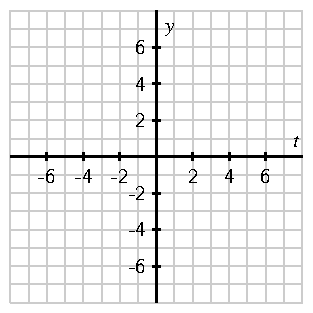
\includegraphics[width=1\linewidth]{images/exp-log-blank-axes}

\end{enumerate}
%
\end{exploration}

%
%
%\typeout{************************************************}
%\typeout{Subsection 3.4.1 The base-\(b\) logarithm}
%\typeout{************************************************}
%
\section{$\log_b$ or logarithms in general}
 In the previous sections, we looked at two specific (and the most common) types of logarithms, base-10 and natural log. In order to fully discuss logarithms, we need to talk about logarithms in general with any base. Let $b>1$. Because the function $y=f(t)=b^t$ has an inverse function, it makes sense to define its inverse like we did when $b=10$ or $b=e$. The base-$b$ logarithm, denoted $\log_{b}(y)$ is defined to be the power to which we raise $b$ to get $y$. 

\[
\log_{b}(y)=t
\]
\[
y=f(t)=b^t
\]

\begin{example} Evaluate the following base-$b$ logarithms.
\begin{enumerate}
\item $\log_{2}(8)$
\item $\log_{5}(25)$
\end{enumerate}
\begin{explanation}
\begin{enumerate}
\item 
\begin{align*}
\log_{2}(8)&=\log_{2}(2^3)
\log_{2}(8)&= 3
\end{align*}

\item
\begin{align*} 
\log_{5}(25)&=\log_{5}(5^2)
\log_{5}(25) & = 2
\end{align*}

\end{enumerate}
\end{explanation}
\end{example}

%
%
%\typeout{************************************************}
%\typeout{Subsection 3.4.3 \(f(t) = b^t\) revisited}
%\typeout{************************************************}
%
\section{Revisiting $f(t) = b^t$}

In earlier sections, we saw that that function \(f(t) = b^t\) plays a key role in modeling exponential growth and decay, and that the value of \(b\) not only determines whether the function models growth (\(b \gt 1\)) or decay (\(0 \lt b \lt 1\)), but also how fast the growth or decay occurs.  Furthermore, once we introduced the natural base \(e\), we realized that we could write every exponential function of form \(f(t) = b^t\) as a horizontal scaling of the function \(E(t) = e^t\) by writing%
\begin{equation*}
b^t = f(t) = E(kt) = e^{kt}
\end{equation*}
for some value \(k\).  Our development of the natural logarithm function in the current section enables us to now determine \(k\) exactly.%
\begin{example}

Determine the exact value of \(k\) for which \(f(t) = 3^t = e^{kt}\).%

\begin{explanation} Since we want \(3^t = e^{kt}\) to hold for every value of \(t\) and \(e^{kt} = (e^k)^t\), we need to have \(3^t = (e^k)^t\), and thus \(3 = e^k\).  Therefore, \(k\) is the power to which we raise \(e\) to get \(3\), which by definition means that \(k = \ln(3)\).%
\end{explanation}
\end{example}

In modeling important phenomena using exponential functions, we will frequently encounter equations where the variable is in the exponent, like in the example where we had to solve \(e^k = 3\).  It is in this context where logarithms find one of their most powerful applications.  
\begin{example}
Solve each of the following equations for the exact value of the unknown variable.  If there is no solution to the equation, explain why not.%

\begin{enumerate}[label=\alph*.]
\item
\(e^t = \frac{1}{10}\)%
\item
\(5e^{t}=7\)%
\item
\(\ln(t) = -\frac{1}{3}\)%
\item
\(e^{1-3t} = 4\)%
\item
\(2\ln(t) + 1 = 4\)%
\item
\(4 - 3e^{2t} = 2\)%
\item
\(4 + 3e^{2t} = 2\)%
\item
\(\ln(5 - 6t) = -2\)%
\end{enumerate}
\begin{explanation}
\begin{enumerate}[label=\alph*.]
\item
\begin{align*}
e^t &= \frac{1}{10}\\
\ln(e^t) &= \ln{\left(\frac{1}{10}\right)}\\
t&=\ln{\left(\frac{1}{10}\right)}
\end{align*}
\item
\begin{align*}
5e^{t}&=7\\
e^{t}&=\frac{7}{5}\\
\ln{(e^{t})}&=\ln{\left(\frac{7}{5}\right)}\\
t &=\ln{\left(\frac{7}{5}\right)}
\end{align*}
\item
\begin{align*}
\ln(t) &= -\frac{1}{3}\\
e^{\ln(t)} &=e^{-\frac{1}{3}}\\
t &=e^{-\frac{1}{3}}
\end{align*}
\item

\begin{align*}
e^{1-3t} &= 4\\
\ln(e^{1-3t}) &= \ln(4)\\
1-3t &= \ln(4)\\
-3t &= \ln(4)-1\\
t &= \frac{\ln(4)-1}{-3}
\end{align*}

\item
\begin{align*}
2\ln(t) + 1 &= 4\\
2\ln(t) &= 3\\
\ln(t) &= \frac{3}{2}\\
e^{ln(t)} &= e^{\frac{3}{2}}\\
t &= e^{\frac{3}{2}}
\end{align*}
\item
\begin{align*}
4 - 3e^{2t} &= 2\\
-3e^{2t} &= -2\\
e^{2t} &= \frac{2}{3}\\
\ln(e^{2t}) &= \ln\left({\frac{2}{3}}\right)\\
2t &= \ln\left({\frac{2}{3}}\right)\\
t &= \frac{\ln\left({\frac{2}{3}}\right)}{2}
\end{align*}
\item
\begin{align*}
4 + 3e^{2t} &= 2\\
3e^{2t} &= -2\\
e^{2t} &= \frac{-2}{3}\\
\end{align*}
No solution, because $\frac{-2}{3}$ is outside of the range of $e^{2t}$
\item
\begin{align*}
\ln(5 - 6t) &= -2\\
\ln(5 - 6t) &= -2\\
e^{\ln(5-6t)} &=e^{-2}\\
5-6t &=e^{-2}\\
t &=\frac{e^{-2}-5}{-6}
\end{align*}
\end{enumerate}
\end{explanation}
%
\end{example}

%
%
%\typeout{************************************************}
%\typeout{Subsection 3.4.4 Summary}
%\typeout{************************************************}
%

\begin{summary}
\begin{enumerate}
\item
The base-\(10\) logarithm of \(y\), denoted \(\log_{10}(y)\) is defined to be the power to which we raise \(10\)  to get \(y\).  For instance, \(\log_{10}(1000) = 3\), since \(10^3 = 1000\).  The function \(L(y) = \log_{10}(y)\) is thus the inverse of the powers-of-\(10\) function, \(P(t) = 10^t\).%
\item
The natural logarithm \(N(y) = \ln(y)\)  differs from the base-\(10\) logarithm in that it is the logarithm with base \(e\) instead of \(10\), and thus \(\ln(y)\) is the power to which we raise \(e\) to get \(y\).  The function \(N(y) = \ln(y)\) is the inverse of the natural exponential function \(E(t) = e^t\).%
\item
The natural logarithm often enables us solve an equation that involves \(e\) to some unknown quantity.  For instance, to solve \(2e^{3t-4} + 5 = 13\), we can first solve for \(e^{3t-4}\) by subtracting \(5\) from each side and dividing by \(2\) to get%
\begin{equation*}
e^{3t-4} = 4\text{.}
\end{equation*}
This last equation says ``\(e\) to some power is \(4\)''.  We know that it is equivalent to say%
\begin{equation*}
\ln(4) = 3t-4\text{.}
\end{equation*}
Since \(\ln(4)\) is a number, we can solve this most recent linear equation for \(t\).  In particular, \(3t = 4 + \ln(4)\), so%
\begin{equation*}
t = \frac{1}{3}(4 + \ln(4))\text{.}
\end{equation*}
%
\end{enumerate}
\end{summary}


\end{document}
